\section{Introduction}

Quantum theory is often regarded as one of the most inaccessible scientific disciplines.
Its introduction to university students is typically delayed to the later years of their training due to the complexity of the mathematical and physical content and a substantive reliance on symbolic thinking within the Hilbert space formalism~\cite{Marshman2016difficultqoperators}.
Meanwhile, the last few decades have seen multiple proposals to teach quantum science to students as young as secondary schoolers~\cite{stadermann2019analysis, michelini2000proposal, bitzenbauer2020new, escalada2004student}. However, despite the progress made by recent advancements~\cite{economou2022hello, walsh2021piloting, perry2019quantum, hughes2022teaching, davis2022quantum}, most current approaches to teaching quantum concepts at both high school and university levels remain hampered by a significant number of advanced mathematical prerequisites, including matrix multiplication, complex numbers, and probability theory. 
A recent survey of 28 introductory undergraduate courses in quantum information science, intended for physicists, computer scientists, and mathematicians, found that 75\% had linear algebra as a prerequisite~\cite{meyer2022interdisciplinary}.
Furthermore, instructors interviewed as part of the survey reported that their students had difficulty both at the mathematical level---linear algebra and complex numbers\footnote{Presently only part of the Further Maths syllabus in the UK.\newline \newline } being the main barriers to entry---and at the physical level.
% \textcolor{magenta}{Sieglinde note: ¿Do we have a copy of the latest syllabus? in 1998, there was an option to do further/advanced maths and standard maths. Only further maths covered complex numbers, so many had not seen complex numbers until they had joined university. What is the case now?  }
% \textcolor{magenta}{ The next paragraph about applying tools with conceptual understanding makes sense if we can have a way of distinguishing that they correctly applying the spider rules without conceptual understanding  vs with conceptual understanding. How would that be done?}
It has also been reported in the literature that students in quantum mechanics courses are ``often able to apply mathematical tools without a corresponding conceptual understanding''~\cite{baily2010teaching}---a learning outcome likely to have its roots in a historically widespread `shut up and calculate' culture within the quantum sciences~\cite{johansson2018shut,kaiser2014shut}.

The expectation for students to be proficient in such mathematical topics is carried into early efforts to teach quantum computing at the high school level~\cite{perry2019quantum}.
However, teaching strategies that purposefully avoid formal mathematical tools are reportedly associated with learning difficulties and misconceptions~\cite{krijtenburg2017insights}.
Hence, the educational challenge is to reform the teaching of quantum science by (1) reducing the complexity of the abstract mathematical formalism~\cite{bouchee2022towards}, while (2) enhancing the conceptual understanding and (3) maintaining a high level of scientific rigour.

The development of categorical quantum mechanics~\cite{abramsky2009categorical} in the early 2000s showed that an alternative approach to introductory quantum education was possible.
Diagrammatic methods were first introduced in 2005 at the University of Oxford, enabling quantum mechanical reasoning ``using only pictures of lines, squares, triangles and diamonds''~\cite{coecke2006kindergarten}, i.e. with visual, yet formal, tools.
% \textcolor{magenta}{ The sentence following this note is a little hard to read. Could it be rewritten into two shorter sentences? }
Such methods were introduced as the graphical counterpart to strongly compact closed categories, a kind of algebraic structure introduced shortly before~\cite{abramsky2004categorical}.
But the tongue-in-cheek title of the later work~\cite{coecke2006kindergarten}, ``Kindergarten Quantum Mechanics", clearly hinted at the possibility of future educational benefits for younger audiences.

The term ``Quantum Picturalism'' (QP) was coined in 2009~\cite{ContPhys}, when it was also suggested that---in the longer term and subject to further development---QP could make quantum physics accessible to a wider audience beyond university-level physics students. Specifically, it would remove the requirement to have a prerequisite in linear algebra and complex numbers, thus also making the concepts accessible to a younger high school audience. 
A first experiment in this regard was already sketched in~\cite[\S6]{ContPhys}, while a second experimental draft can be found in \cite{exp1}.



QP effects a paradigm shift in how quantum physics is understood and practiced using visually intuitive but mathematically rigorous diagrams, called string diagrams. These diagrams are interdisciplinary, having applicability not only in quantum physics but also in areas such as machine learning, control systems, electronics, game theory, linguistics, control theory etc. Therefore, these diagrams help forge unforeseen connections between disparate areas of STEM. One example is the emerging area of quantum natural language processing, which came into being by drawing an analogy between quantum physics and language.
Innovation occurs when subjects with apparently no connection talk to one another. This methodology (QP) shifts the focus towards a network mindset which fosters innovation.

The use of pictorial representations has a rich history in educational implementations, with extensive evidence thoroughly explored~\cite{tversky2004semantics}. There has been a major focus on the function of instructional pictures as valuable support for, or as an alternative to, both text and symbolic reasoning \cite{bobek2016creating, mielicki2015affordances, herrlinger2017pictures}
with evidence suggesting that visual aids like diagrams enhance learning by providing intuitive explanations, improving memory retention, and catering to diverse learning styles~ \cite{verdi1997organized}. A common way of using visual aids is to simplify complex concepts, while promoting creativity and problem-solving skills. Indeed, there is a growing interest in integrating visual aids into educational implementations, endorsed by modern pedagogical approaches, to foster enriched learning experience and enhance scientific thinking~\cite{mayer2005cambridge, carney2002pictorial, fan2015drawing}.
% \textcolor{cyan}{May need more refs here.} \textcolor{orange}{Better now?}
% \textcolor{cyan}{Does \cite{tversky2004semantics} belong here?}

Consistent with this notion, we claim that the entirely visual nature of QP enhances understanding of quantum theory by lowering the technical barrier, making the topic suitable for a high-school level introduction.
Contrary to visual aids such as multimedia and schematic diagrams (flowcharts, mindmaps, etc.), QP is a mathematically sound diagrammatic method, stemming from a well-established lineage of academic research on ``graphical calculi''~\cite{coecke2022kindergarden}. Furthermore, QP can be used as a self-contained language to describe quantum theory, eliminating the need for informal explanations or additional formal backing: it inherits all the educational benefits of visual approaches while also doubling as a descriptive and computational tool.
The rapidly increasing adoption of QP by both academia and the quantum industry further shows that such advantages come at no expense of scientific rigour or cutting-edge applicability.

\begin{figure*}[ht]
\centering
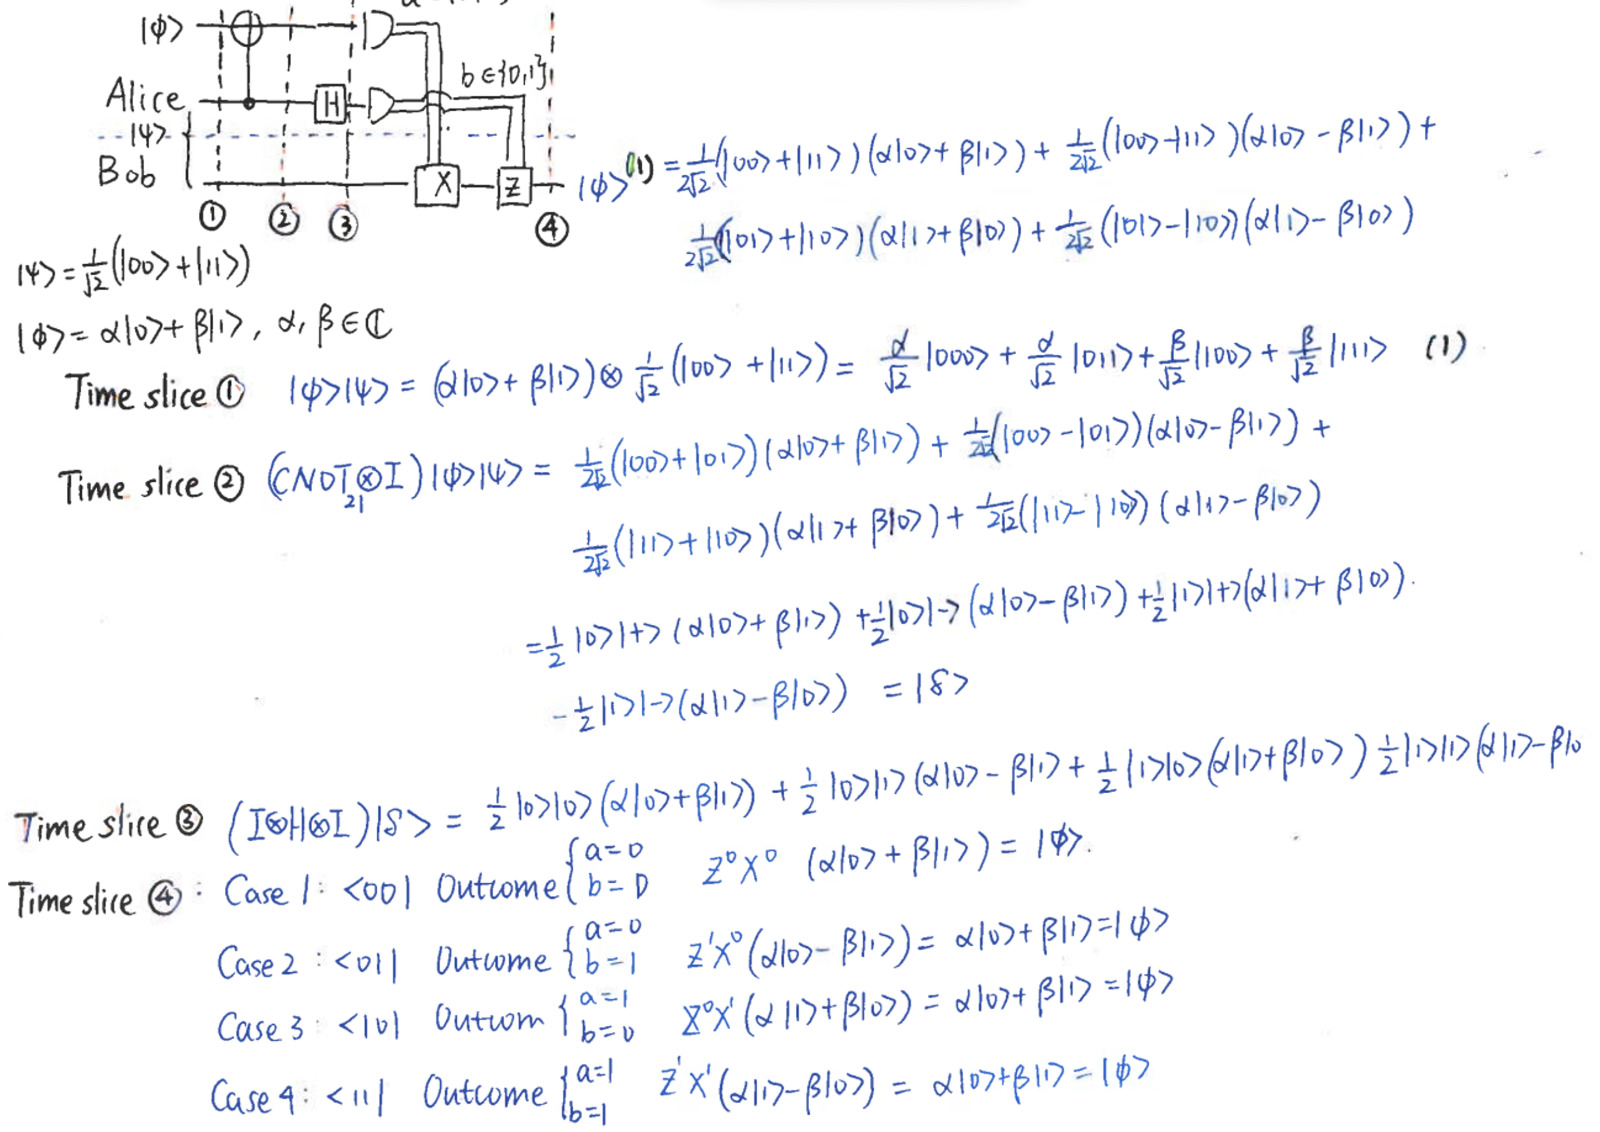
\includegraphics[width=0.69\textwidth]{Sections/pictures/teleportation-learning.jpg}
\caption{
Calculations in bra-ket notation by Master's student Sarah Meng Li from the University of Waterloo, demonstrating the correctness of the quantum teleportation protocol as part of their graduate course QIC 710: Intro to Quantum Information Processing. The figure exemplifies how the Hilbert space formalism produces a much more arcane description of the quantum teleportation protocol, as opposed to the intuitive diagrammatic version of Fig. \ref{fig:diagrammatic-reasoning-teleportation-steps}.
}
\label{fig:teleportation-learning}
\end{figure*}

Contrary to the prevailing belief that symbolic mathematics is the language of physics, we posit that QP offers an approach to quantum theory that is superior for teaching and everyday practice.

Here, we aim to demonstrate how QP provides learners with effective tools for solving complex problems; and therefore it fosters engagement, improves self-confidence, builds motivation, and incorporates fun into the learning process. It is anticipated that such benefits will persist even in experiments where age, cognitive ability, science background, and attitude towards scientific topics are controlled for.

In response to the increased demand top-down through calls for workforce development, and bottom-up by students, recent years have seen growth of initiatives to teach quantum information science, quantum computing, and quantum mechanics to high school students~\cite{QxQ,OxPhys,IQCqsys,walsh2021piloting,economou2020teaching}.
Students can be attracted to quantum through games and interactive tools~\cite{seskir2022quantumgames, lacour2022vqol, Migdal2022qflytrap, chungyuan2022, Marshman2022, entanglementball2021}, programming~\cite{mykhailova2022, salehiseskir2022, qiskittextbook2021}, collaboration~\cite{khodaeifaal2022, maldonadoromo2022}, and art~\cite{quantumatlas,uchicago2022multidisciplinary}.
Likewise, various strategies have been developed to teach quantum theoretical concepts \cite{hoekzema2007particle, boe2023secondary, huseby2019observation, di2020development, rudolph2017, epiqc2020reversibility}.

There is an open debate as to which features best contribute to improving students' understanding of the subject matter~\cite{krijtenburg2017insights, greca2003does}.
However, the more formal approaches typically rely on symbolic mathematical foundations, using diagrams for descriptive and/or conceptual purposes rather than as the primary substrate for their delivery of knowledge.
In investigating the efficacy of QP as a teaching approach, we establish relevant baselines and gather experiential evidence for future studies in this area.

In this paper, we fully detail QP as a method to teach quantum theory to high school students, without prior exposure to the associated physics background nor the traditional mathematical prerequisites.

We introduce QP in Section~\ref{sec:QP}, and provide the details of a pilot experiment and evaluation methodology to test the efficacy of QP in education in Section~\ref{sec:xpmt}, followed by discussion in Section~\ref{sec:discuss}.
This adheres to the tradition in education sciences of preregistering experiments prior to their being conducted, to receive feedback on the methodology and to safeguard against irresponsible analysis of the data.
